\section{TMVA Quick Start}
\label{sec:quickstart}

To run TMVA it is not necessary to know much about its concepts or to understand 
the detailed functionality of the multivariate methods. Better, just begin 
with the quick start tutorial given below.

Classification and regression analyses in TMVA have similar training, testing and 
evaluation phases, and will be treated in parallel in the following. 

\subsection{How to download and build TMVA}
\label{sec:download}

TMVA is built upon ROOT (\urlsm{http://root.cern.ch/}), so that for TMVA to run ROOT must be 
installed. Since ROOT version 5.11/06, TMVA
comes as integral part of ROOT and can be used from the ROOT prompt 
without further preparation. For older ROOT versions 
or {\em if the latest TMVA features are desired}, the TMVA source code can either be \href{http://sourceforge.net/project/showfiles.php?group_id=152074}{downloaded}
as a gzipped tarfile from Sourceforge.net\index{Download!from Sourceforge.net}
.%or directly be checked out via (anonymous) SVN from the ROOT repository. 
%\begin{codeexample}
%\begin{tmvacode}
%~> svn co https://root.cern.ch/svn/root/branches/dev/tmvapatches/V04-01-00 \ 
%tmva_4.1.0
%\end{tmvacode}
%\caption[.]{\codeexampleCaptionSize DEPRECATED! (root has moved recently to Git and ...for the moment
%we don't know how to get the latest TMVA version (only) from the Git repository.) And we don't know how
%long the SVN repository is still available: Source code download via SVN. The latest version 
%         (SVN trunk) can be always be obtained by typing:
%         \spacecode{svn co https://root.cern.ch/svn/root/trunk/tmva}. For the latest TMVA 
%         version see \url{http://root.cern.ch/} or \url{http://tmva.sourceforge.net/}.}
%\end{codeexample}
Since we do not provide prebuilt libraries for any platform,
the library must be built by the user (easy -- see below).
While the source code is known to compile with VisualC++ on Windows (which is
a requirement for ROOT), we do not provide project support for this platform yet.
For Unix and most Linux flavours custom Makefiles\index{Makefile} are provided 
with the TMVA distribution, so that the library can be built by typing:
\begin{codeexample}
\begin{tmvacode}
~> cd tmva
~/tmva> make 
~/tmva> cd test
~/tmva/test> source setup.sh # for c-shell family: source setup.csh
\end{tmvacode}
\caption[.]{\codeexampleCaptionSize Building the TMVA library under Linux/Unix using the provided
         Makefile. The \code{setup.[c]sh} script must be executed to 
         ensure the correct setting of symbolic links and library paths required by TMVA.}
\end{codeexample}
After compilation, the library \code{tmva/lib/libTMVA.1.so} should be present.

If you run TMVA in a working directory other than \code{~/tmva/test}, then you
simply need to copy the \code{setup.[c]sh} file into your work directory and ``source'' it
while giving it as an argument the TMVA installation directory:

\begin{codeexample}
\begin{tmvacode}
~> cd MyWorkDir
~/MyWorkDir> cp ~/tmva/test/setup.[c]sh . 
~/MyWorkDir> source setup.[c]sh <Your TMVA installation path>
\end{tmvacode}
\caption[.]{\codeexampleCaptionSize Using the built TMVA library under Linux/Unix from an arbritrary work directory. The \code{setup.[c]sh <pathToYourTMVAInstallation>} script must be executed to 
         ensure the correct setting of symbolic links and library paths required by TMVA.}
\end{codeexample}

\subsection{Version compatibility}
\label{sec:intro:compat}

TMVA can be run with any ROOT version equal or above v5.08\index{ROOT!compatibility}.
The few occurring conflicts due to ROOT source code evolution after v5.08 are 
intercepted in TMVA via C++ preprocessor conditions.

\subsection{Avoiding conflicts between external TMVA and ROOT's internal one}

A ROOT installation typcially comes a TMVA version already.
To use a more recent version of TMVA than the one present in the local ROOT 
installation, one needs to download the desired TMVA release as described above,
compile it against the local ROOT version and make sure the newly built library 
\code{tmva/lib/libTMVA.1.so} is used instead of ROOT's internal one.
While executing the \code{setup.[c]sh} script is usually sufficient to ensure the latter,
on MAC OSX systems it may be neccessary to load the library exlicitly when running TMVA in CINT:  
\code{gSystem}{\tt ->}\code{Load("tmva/lib/libTMVA.1")}. This can be done 
directly in the macro or in a file that is automatically loaded at the start 
of CINT (for an example, see the files \code{.rootrc} and \code{TMVAlogon.C} 
in the \code{tmva/test/} directory).  When running TMVA in an executable, 
the corresponding shared library needs to be linked.
Once this is done, ROOT's own \code{libTMVA.so} library will not be invoked anymore.

\subsection{The TMVA namespace}
\label{sec:quickstart:namespace}

All TMVA classes are embedded in the namespace \code{TMVA}. For interactive access, or 
use in macros the classes must thus be preceded by \code{TMVA::}, or one may use the 
command \code{using} \code{namespace} \code{TMVA} instead. 

\subsection{Example jobs\index{Examples}}
\label{sec:examplejob}

TMVA comes with example jobs for the training phase (this phase actually 
includes training, testing and evaluation) using the TMVA {\em Factory}\index{Factory}, 
as well as the application of the training results in a classification or regression analysis
using the TMVA {\em Reader}\index{Reader}. The training examples are
\code{TMVAClassification}\index{TMVAClassification},
\code{TMVAMulticlass.C}\index{TMVAMulticlass} and
\code{TMVARegression}\index{TMVARegression}, and the application examples are 
\code{TMVAClassificationApplication}\index{TMVAClassificationApplication},
\code{TMVAMulticlassApplication.C}\index{TMVAMulticlassApplication} and
\code{TMVARegressionApplication}\index{TMVARegressionApplication}.

The above macros (extension \code{.C})
are located in the directory \code{tmva/test/}. 

All examples are also provided in form of C++ executables
(replace \code{.C} by \code{.cxx}). To build the executables, go to
\code{tmva/test/}, type \code{make} and then simply execute them by typing
\code{./TMVAClassification}, \code{./TMVAMulticlass} or \code{./TMVARegression} (and similarly for the 
applications). To illustrate how TMVA can be used 
in a python script via PyROOT we also provide the script \code{TMVAClassification.py} located 
in \code{TMVA/python/}, which has the same functionality as the macro \code{TMVAClassification.C}
(the other macros are not provided as python scripts).

\subsection{Running the example}
\label{sec:qs:example}

The most straightforward way to get started with TMVA is to simply run the \code{TMVAClassification.C} 
or \code{TMVARegression.C} example macros. Both use academic toy datasets for training 
and testing, which, for classification, consists of four linearly correlated, Gaussian 
distributed discriminating input variables, with different sample means for signal and 
background, and, for regression, has two input variables with fuzzy parabolic dependence 
on the target (\code{fvalue}), and no correlations among themselves. All 
classifiers are trained, tested and evaluated using the toy datasets in the
same way the user is expected to proceed for his or her own data. It
is a valuable exercise to look at the example file in more detail. Most 
of the command lines therein should be self explaining, and one will easily 
find how they need to be customized to apply TMVA to a real use case.
A detailed description is given in Sec.~\ref{sec:usingtmva}.

The macros automatically fetch the data file from 
the web using the corresponding \code{TFile} constructor, \eg,
\code{TFile::Open("http://root.cern.ch/files/tmva_class_example.root")} (\code{tmva_reg_example.root} for regression). The example %ToDo: insert this code into our example execs and macros. 
ROOT macros can be run directly in the \code{tmva/test/} directory,
or in any designated test directory \code{workdir}, after adding the macro directory 
to ROOT's macro search path:
\begin{codeexample}
\begin{tmvacode}
~/workdir> echo "Unix.*.Root.MacroPath: $ROOTSYS/tmva/test" >> .rootrc
~/workdir> root -l $ROOTSYS/tmva/test/TMVAClassification.C
\end{tmvacode}
\caption[.]{\codeexampleCaptionSize Running the example \code{TMVAClassification.C}.}
\end{codeexample}

It is also possible to explicitly select the MVA methods to be processed: 
\begin{codeexample}
\begin{tmvacode}
~/workdir> root -l $ROOTSYS/tmva/test/TMVAClassification.C\(\"Fisher\"\)
\end{tmvacode}
\caption[.]{\codeexampleCaptionSize Running the example \code{TMVAClassification.C} 
            and processing only the Fisher classifier. Note that
            the backslashes are mandatory. Multiple classifiers are separated by commas.
            The others macros can be 
            called accordingly. }
\end{codeexample}
where the names of the MVA methods are predifined in the macro. 

The training job provides formatted output logging containing analysis information
such as: linear correlation matrices for the input variables, correlation ratios 
and mutual information (see below) between input variables and regression targets,
variable ranking, summaries of the MVA configurations, goodness-of-fit evaluation
for PDFs (if requested), signal and background (or regression target) correlations 
between the various MVA methods, decision overlaps, signal efficiencies
at benchmark background rejection rates (classification) or deviations from target 
(regression), as well as other performance estimators. Comparison between the results
for training and independent test samples provides overtraining validation.
\begin{figure}[p]
  \begin{center}
	  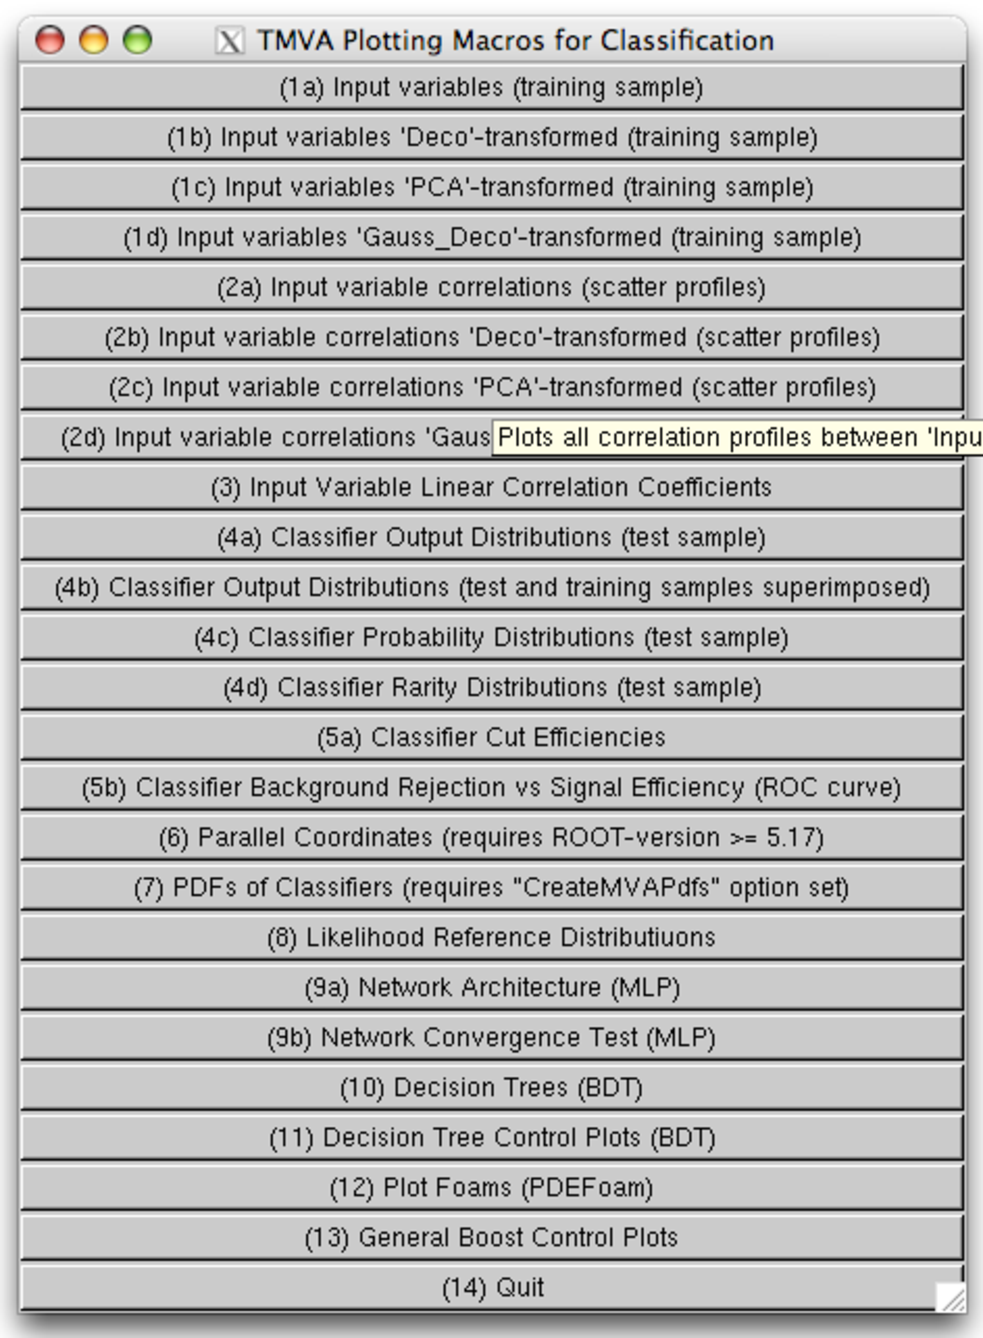
\includegraphics[width=0.47\textwidth]{plots/TMVAGui}\hspace{0.3cm}
	  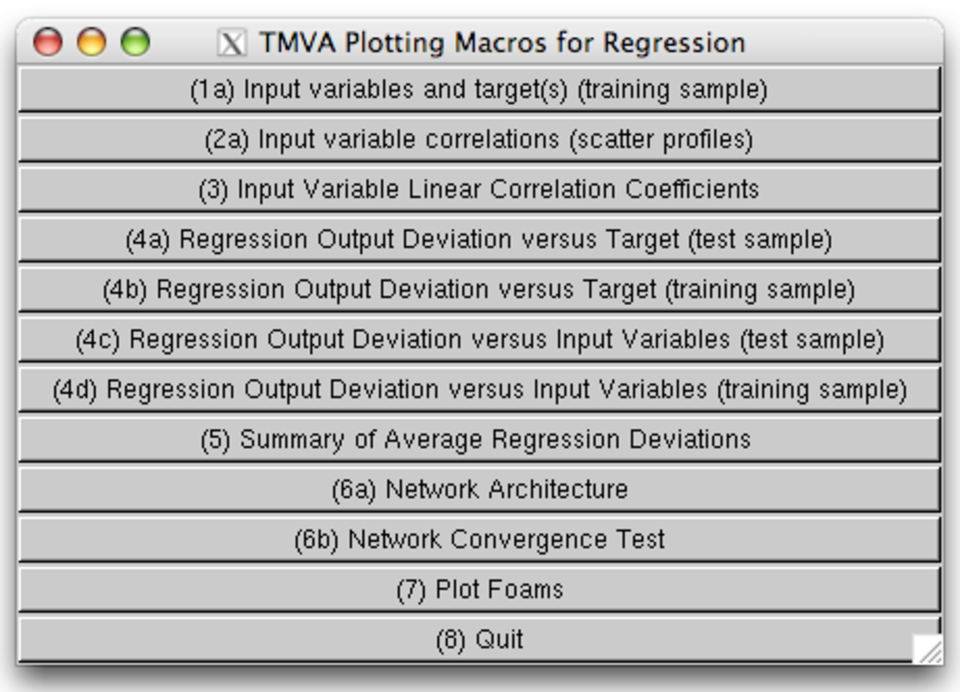
\includegraphics[width=0.47\textwidth]{plots/TMVARegGui}
  \end{center}
  \vspace{-0.1cm}
  \caption[.]{Graphical user interfaces (GUI) to execute  
              macros displaying training, test and evaluation results 
              (\cf\  Tables~\ref{pgr:scripttable1} and \ref{pgr:scripttable2} on page 
              \pageref{pgr:scripttable1}) for classification (left) and regression 
              problems (right). The multiclass classification GUI is similar to the classification GUI,
              where some functionality is not available.
              The classification GUI can be launched manually by executing the script
              {\tt \$}\code{ROOTSYS/tmva/test/TMVAGui.C} in a ROOT 
              session. To launch the multiclass or regression GUIs use the macros \code{TMVARegGui.C}
              or \code{TMVAMultiClassGui.C}, respectively. \\[0.2cm]
              {\footnotesize
              \underline{Classification (left)}. The buttons behave as follows:
              (1a) plots the signal and background 
              distributions of input variables (training sample), (1b--d) the 
              same after applying the corresponding preprocessing transformation of the input 
              variables, (2a--f) scatter plots with superimposed profiles for all 
              pairs of input variables for signal and background and the applied transformations
              (training sample), (3) correlation coefficients 
              between the input variables for signal and background (training sample), 
              (4a/b) signal and background distributions for the trained classifiers (test 
              sample/test and training samples superimposed to probe overtraining), 
              (4c,d) the corresponding probability and Rarity distributions of the classifiers
              (where requested, \cf\  see Sec.~\ref{sec:otherRepresentations}), 
              (5a) signal and background efficiencies and purities versus the cut on the classifier
              output for the expected numbers of signal and background events (before applying the cut) 
              given by the user (an input dialog box pops up, where the numbers are inserted),
              (5b) background rejection versus signal efficiency obtained when cutting 
              on the classifier outputs (ROC curve, from the test sample), (6) plot of so-called
              Parallel Coordinates visualising the correlations among the input variables, and 
              among the classifier and the input variables,  (7--13) show classifier 
              specific diagnostic plots, and (14) quits the GUI. Titles greyed out indicate 
              actions that are not available because the corresponding classifier has not 
              been trained or because the transformation was not requested.\\
              \underline{Regression (right)}. The buttons behave as follows:
              (1--3) same as for classification GUI, (4a--d) show the linear deviations between 
              regression targets and estimates versus the targets or input variables for the 
              test and training samples, respectively, (5) compares the average deviations 
              between target and MVA output for the trained methods, and (6--8) are as for the classification GUI.}
}
\label{fig:tmvagui}
\end{figure}

\subsection{Displaying the results}
\label{sec:displayingResults}

\begin{figure}[!t]
\begin{center}
  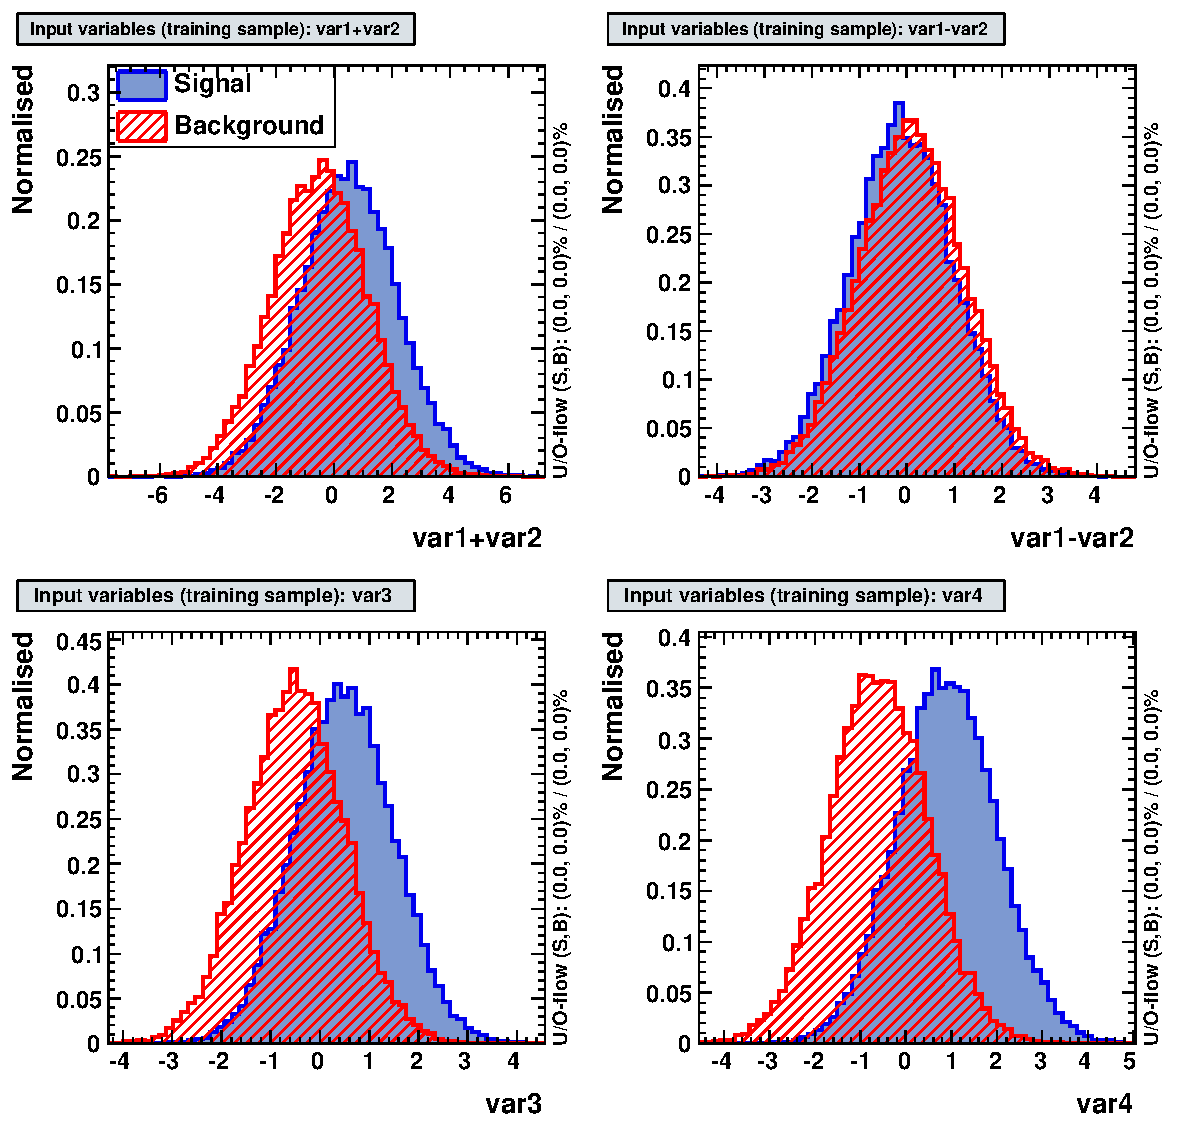
\includegraphics[width=0.8\textwidth]{plots/variables_c1}
\end{center}
  \vspace{-0.5cm}
\caption[.]{Example plots for input variable distributions. The histogram
            limits are chosen to zoom into the bulk of the distributions, which
            may lead to truncated tails. The vertical text on the 
            right-hand side of the plots indicates the under- and overflows.
            The limits in terms of multiples of the distribution's RMS can 
            be adjusted in the user script by modifying the variable
            \code{(TMVA::gConfig().GetVariablePlotting()).fTimesRMS} (\cf\  
            Code Example~\ref{ce:gconfig}). }
\label{fig:usingtmva:variables}
\end{figure}
Besides so-called ``weight'' files containing the
method-specific training results, TMVA also provides a variety of
control and performance plots that can be displayed via a set of ROOT
macros available in {\tt \$}\code{ROOTSYS/tmva/test/}. The macros are summarized in
Tables~\ref{pgr:scripttable1} and \ref{pgr:scripttable2} on 
page~\pageref{pgr:scripttable1}.  At the end of the example jobs a graphical 
user interface (GUI)\index{Graphical user interface (GUI)}
is displayed, which conveniently allows to run these macros (see
Fig.~\ref{fig:tmvagui}).  
 
Examples for plots produced by these macros are given in 
Figs.~\ref{fig:usingtmva:correlations}--\ref{fig:usingtmva:rejBvsS} for a 
classification problem.
The distributions of the input variables for signal and background 
according to our example job are shown in Fig.~\ref{fig:usingtmva:variables}. 
It is useful to quantify the correlations between the input variables.
These are drawn in form of a scatter plot with the superimposed profile for
two of the input variables in Fig.~\ref{fig:usingtmva:correlations} (upper left).  
As will be discussed in Sec.~\ref{sec:dataPreprocessing}, TMVA allows to perform 
a linear decorrelation transformation of the input variables prior to the MVA
training (for classification only). The result of such decorrelation is shown 
at the upper right hand plot of Fig.~\ref{fig:usingtmva:correlations}. The lower 
plots display the linear correlation coefficients between all input variables, 
for the signal and background training samples of the classification example.

Figure~\ref{fig:usingtmva:mvas} shows several classifier output 
distributions for signal and background events based on the test sample. 
By TMVA convention, signal (background) events accumulate at large 
(small) classifier output values. Hence, cutting on the output and retaining
the events with \yMVA larger than the cut requirement selects signal samples
with efficiencies and purities that respectively decrease and increase with 
the cut value. The resulting relations between background rejection versus 
signal efficiency are shown in Fig.~\ref{fig:usingtmva:rejBvsS} for all 
classifiers that were used in the example macro. This plot belongs to the 
class of {\em Receiver Operating Characteristic} (ROC)\index{Receiver 
Operating Characteristic (ROC)} diagrams,
which in its standard form shows the true positive rate versus the false 
positive rate for the different possible cutpoints of a hypothesis test.

As an example for multivariate regression, Fig.~\ref{fig:usingtmva:deviation} displays
the deviation between the regression output and target values for linear and 
nonlinear regression algorithms. 

More macros are available to validate training and response of specific 
MVA methods. For example, the macro \code{likelihoodrefs.C} compares the 
probability density functions used by the likelihood classifier to the normalised 
variable distributions of the training sample. It is also possible to visualize 
the MLP neural network architecture and to draw decision trees (see 
Table~\ref{pgr:scripttable2}).
\begin{figure}[t]
\begin{center}
  \def\thissize{0.40}
  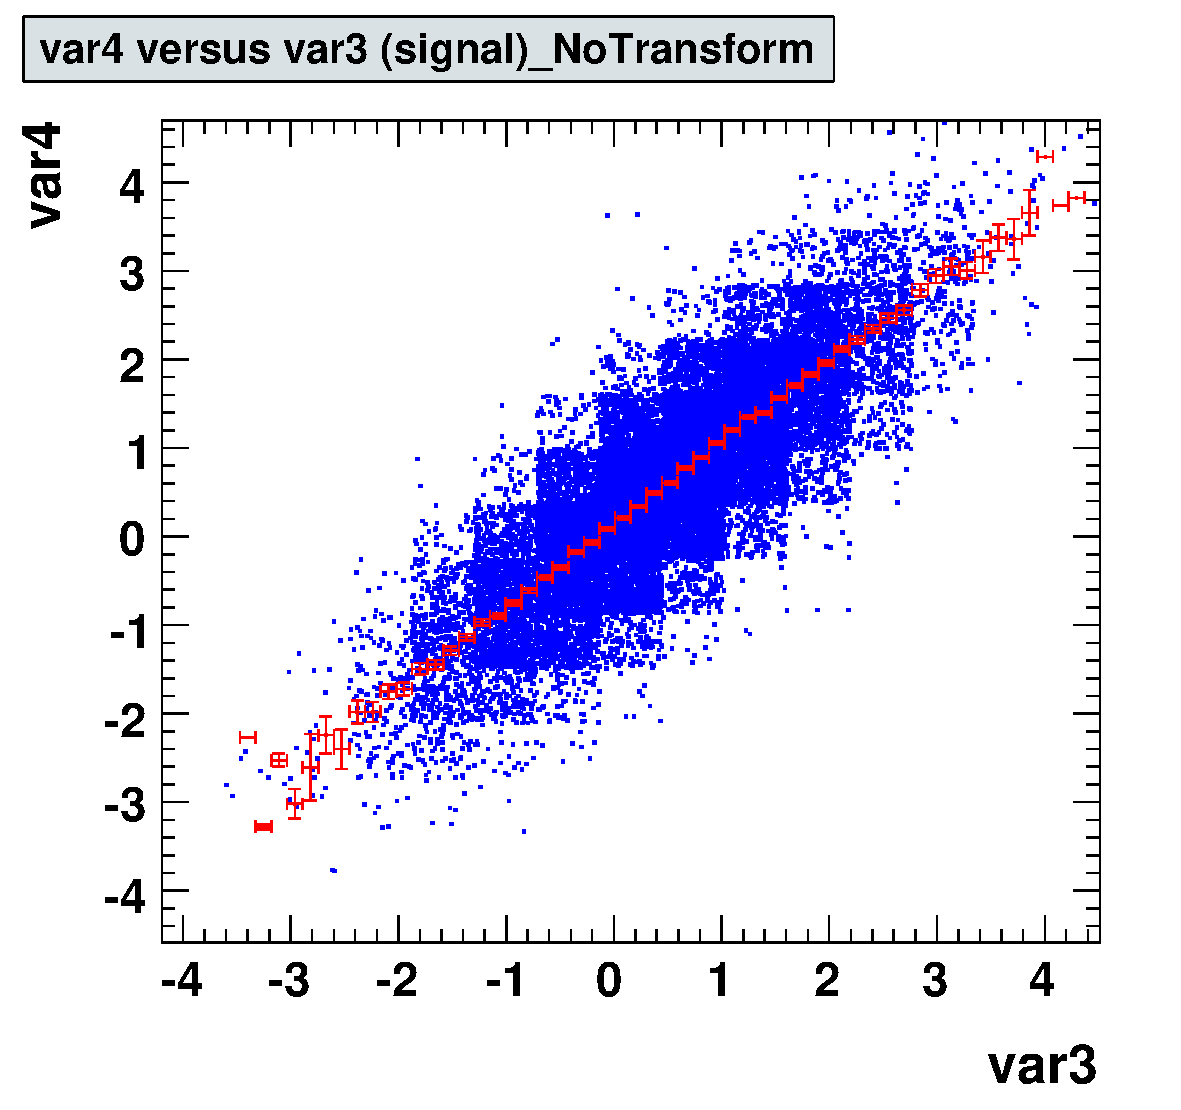
\includegraphics[width=\thissize\textwidth]{plots/correlationscatter__NoTransform_c1}
  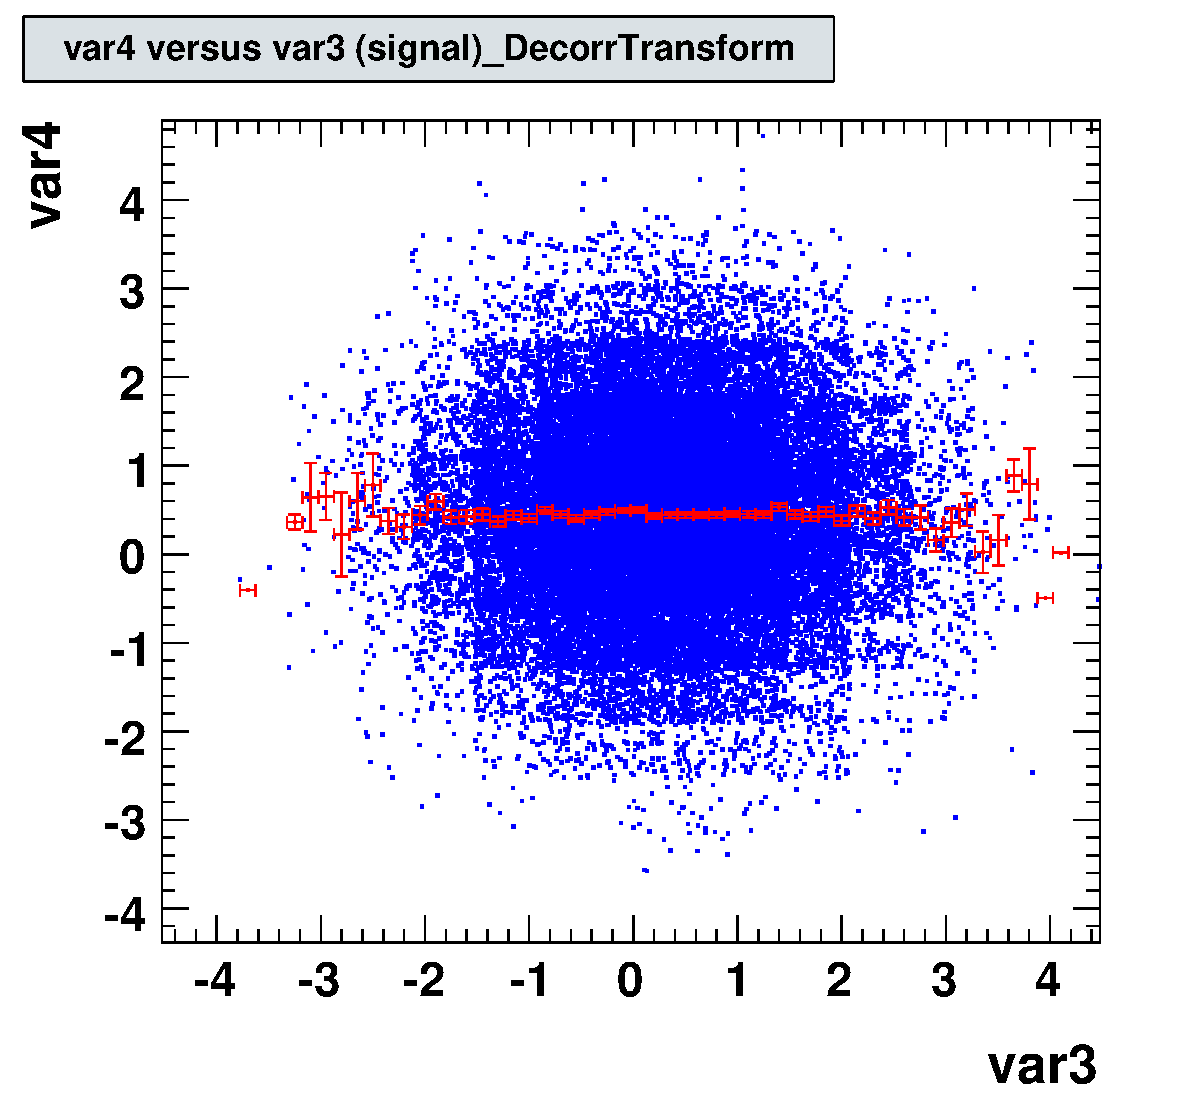
\includegraphics[width=\thissize\textwidth]{plots/correlationscatter__DecorrTransform_c1}

  \vspace{0.2cm}

  \def\thissize{0.40}
  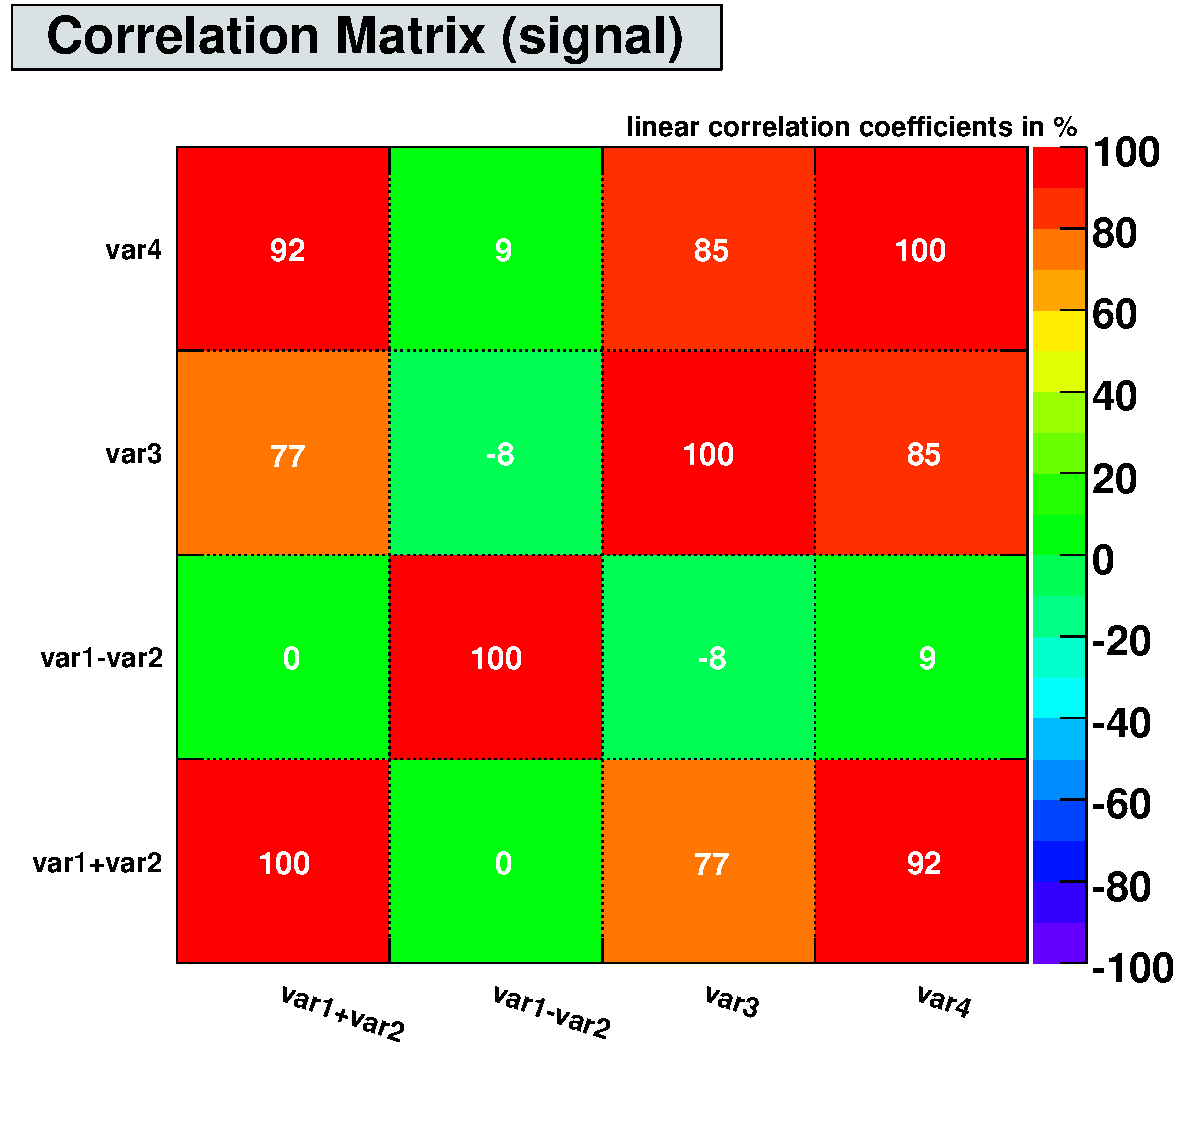
\includegraphics[width=\thissize\textwidth]{plots/CorrelationMatrixS}
  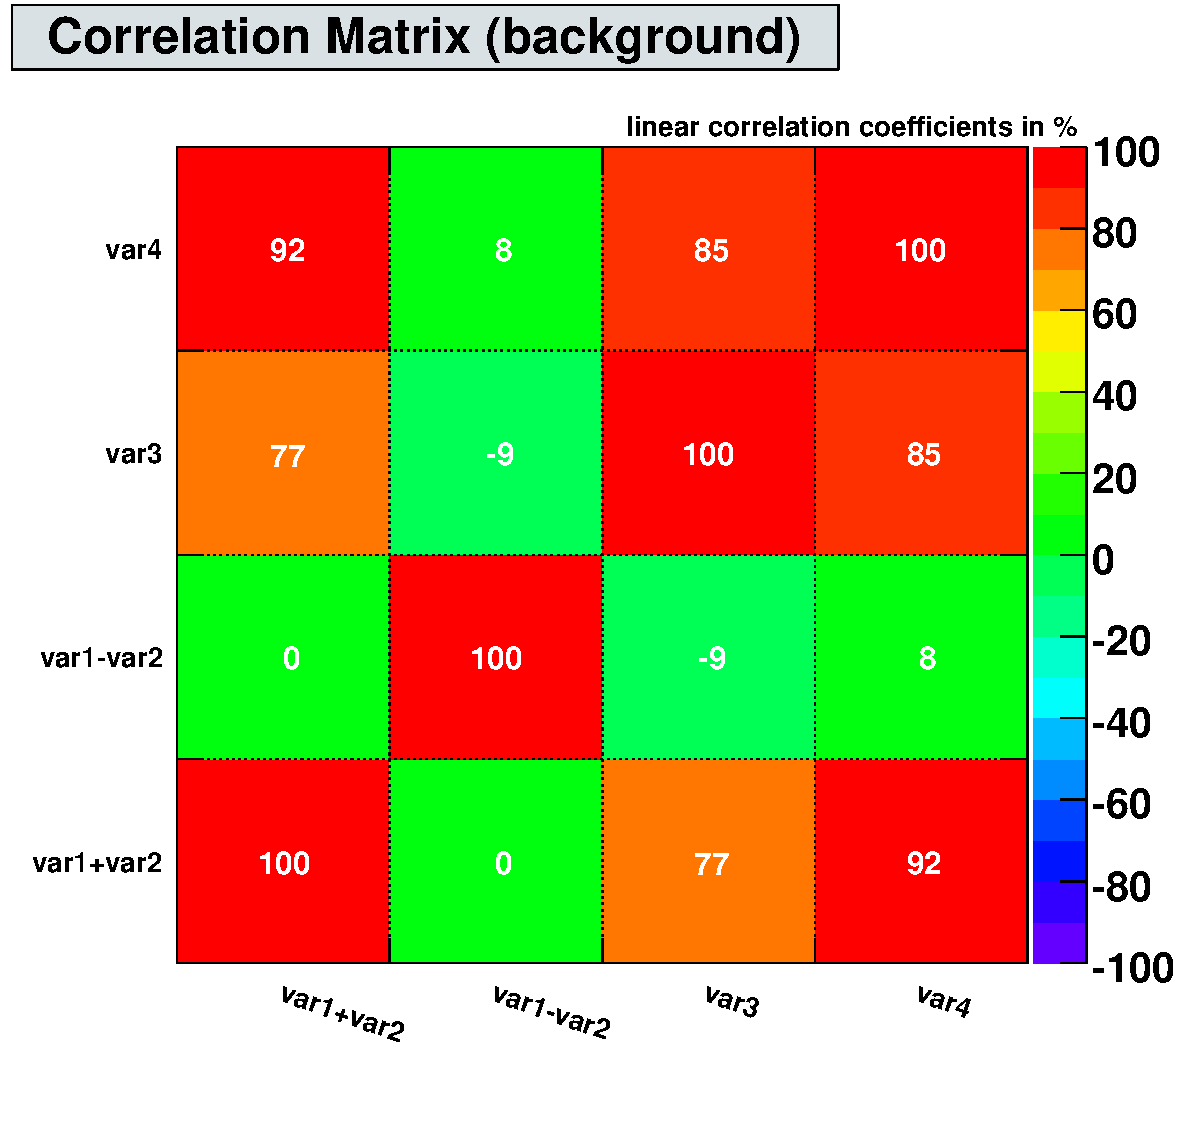
\includegraphics[width=\thissize\textwidth]{plots/CorrelationMatrixB}
\end{center}
\vspace{-0.7cm}
\caption[.]{Correlation between input variables. Upper left: correlations
         between var3 and var4 for the signal training sample. 
         Upper right: the same after applying a linear decorrelation transformation 
         (see Sec.~\ref{sec:decorrelation}). Lower plots: 
         linear correlation coefficients for the signal and background 
         training samples.
}
\label{fig:usingtmva:correlations}
\end{figure}
\begin{figure}[t]
\begin{center}
  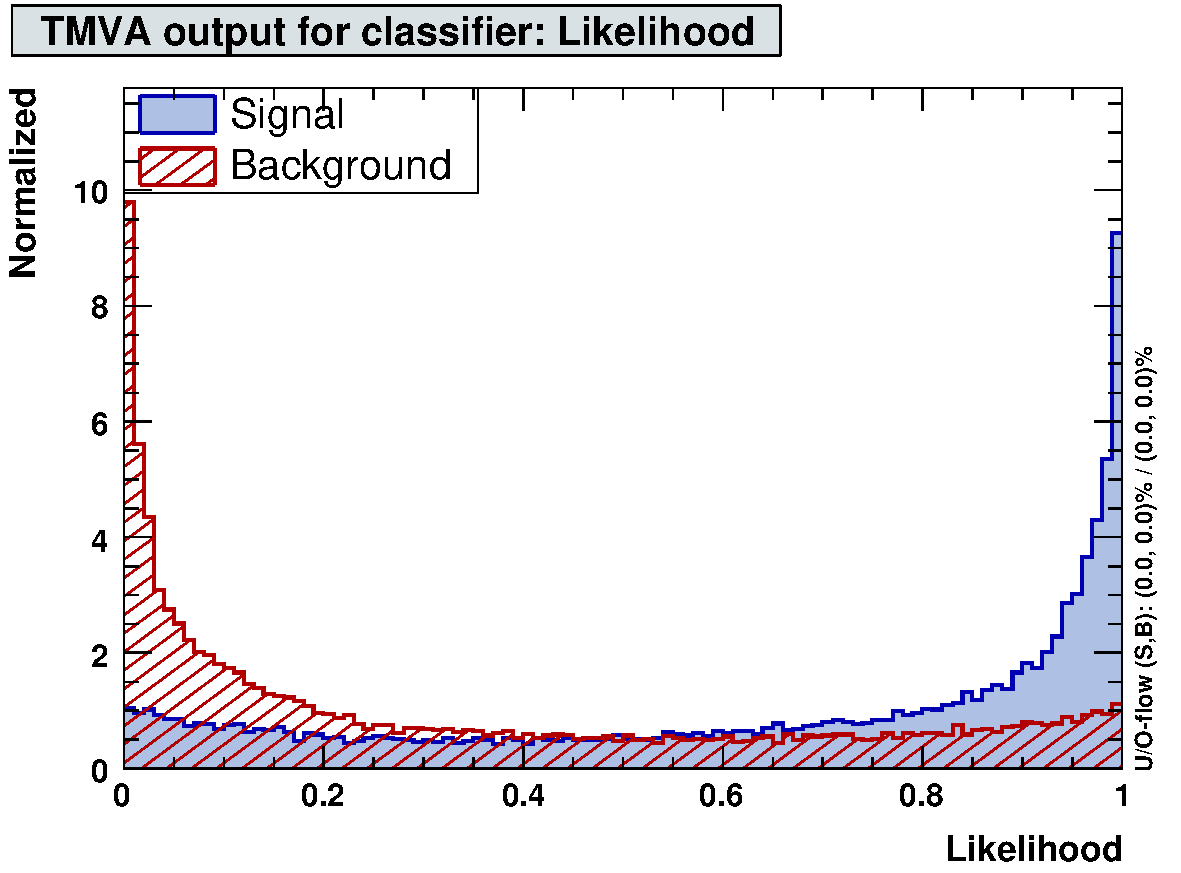
\includegraphics[width=0.50\textwidth]{plots/MVA-Likelihood}
  \hspace{-0.3cm}
  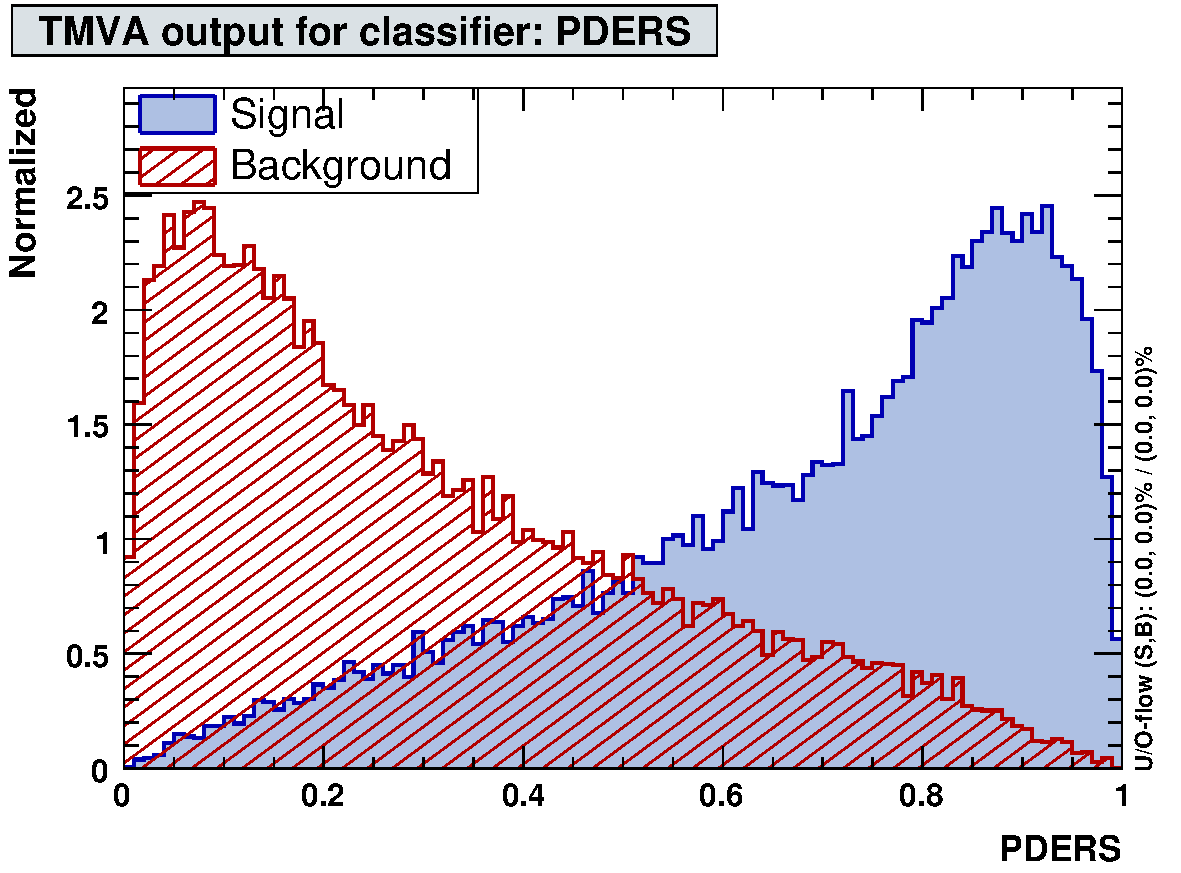
\includegraphics[width=0.50\textwidth]{plots/MVA-PDERS}

  \vspace{0.2cm}

  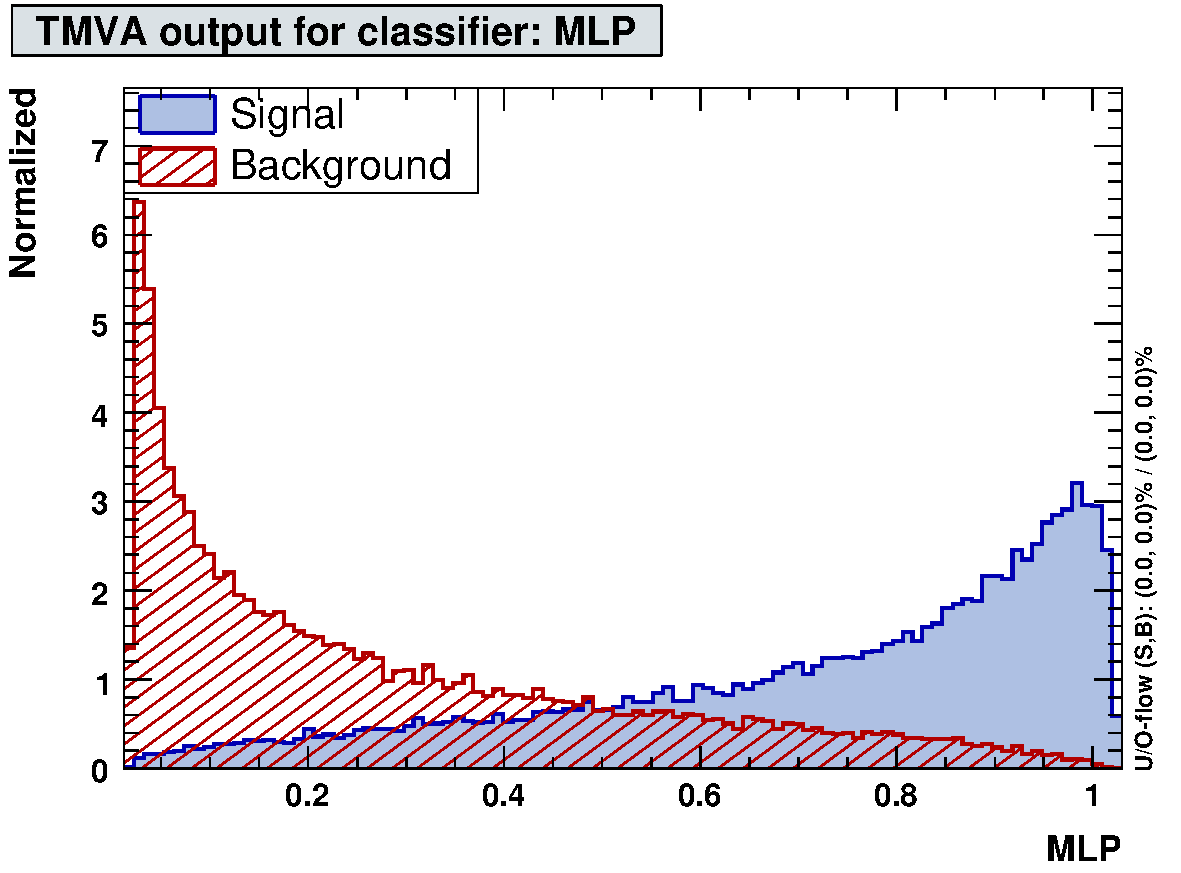
\includegraphics[width=0.50\textwidth]{plots/MVA-MLP}
  \hspace{-0.3cm}
  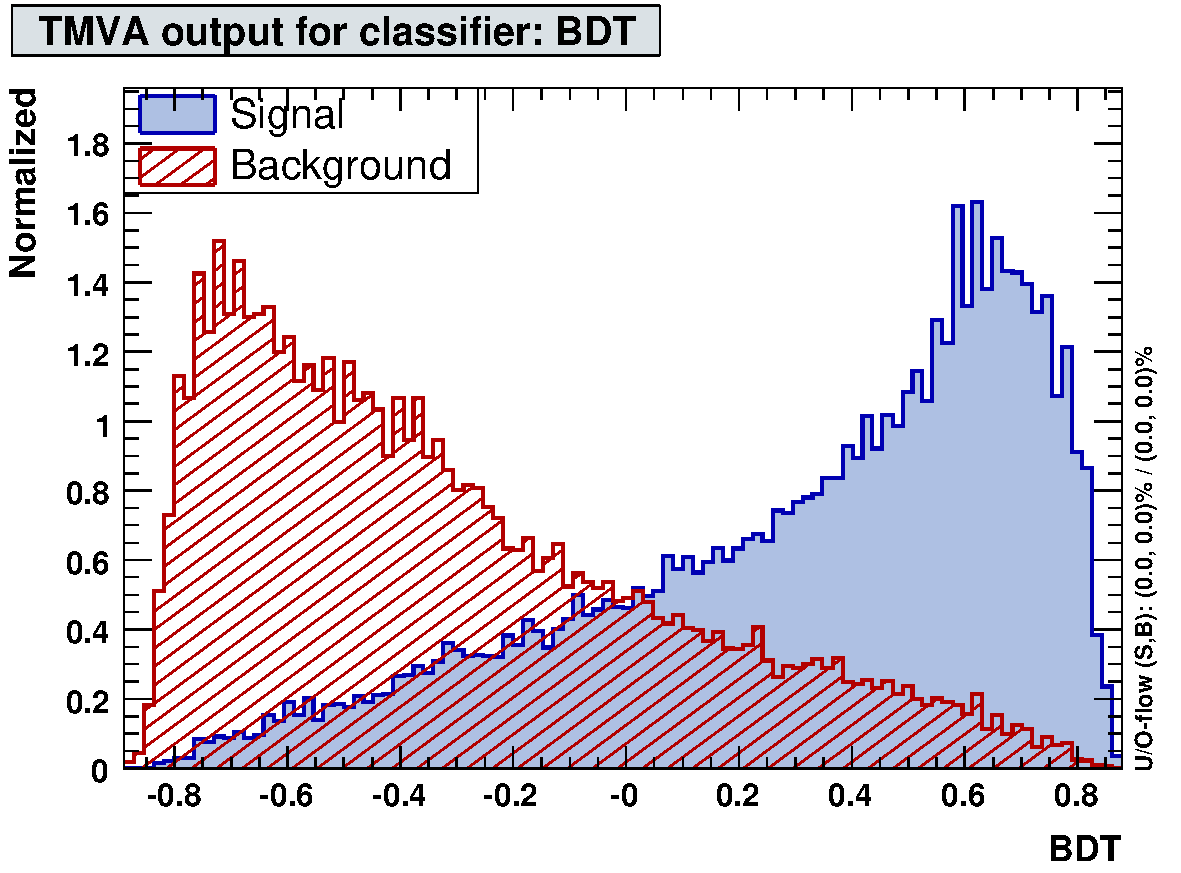
\includegraphics[width=0.50\textwidth]{plots/MVA-BDT}
\end{center}
\vspace{-0.5cm}
\caption[.]{Example plots for classifier output distributions for signal and 
            background events from the academic test sample. Shown are
            likelihood (upper left), PDE range search
            (upper right), Multilayer perceptron (MLP -- lower left) and boosted decision trees.}
\label{fig:usingtmva:mvas}
\end{figure}
\begin{figure}[t]
\begin{center}
  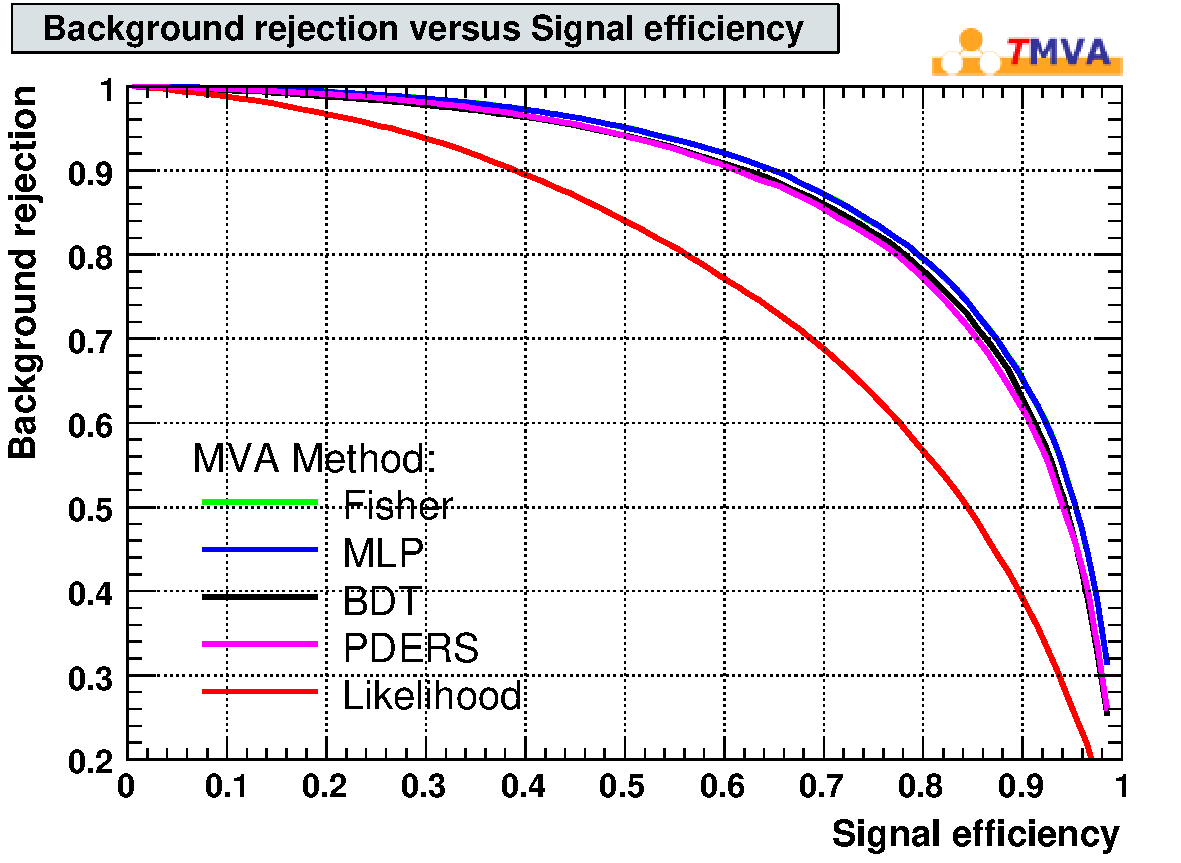
\includegraphics[width=0.65\textwidth]{plots/rejBvsS}
\end{center}
\vspace{-0.5cm}
\caption[.]{Example for the background rejection versus signal efficiency (``ROC curve'') obtained
            by cutting on the classifier outputs for the events of the test sample.
            \index{Performance evaluation!background rejection vs. signal efficiency} }
\label{fig:usingtmva:rejBvsS}
\end{figure}
\begin{figure}[t]
\begin{center}
  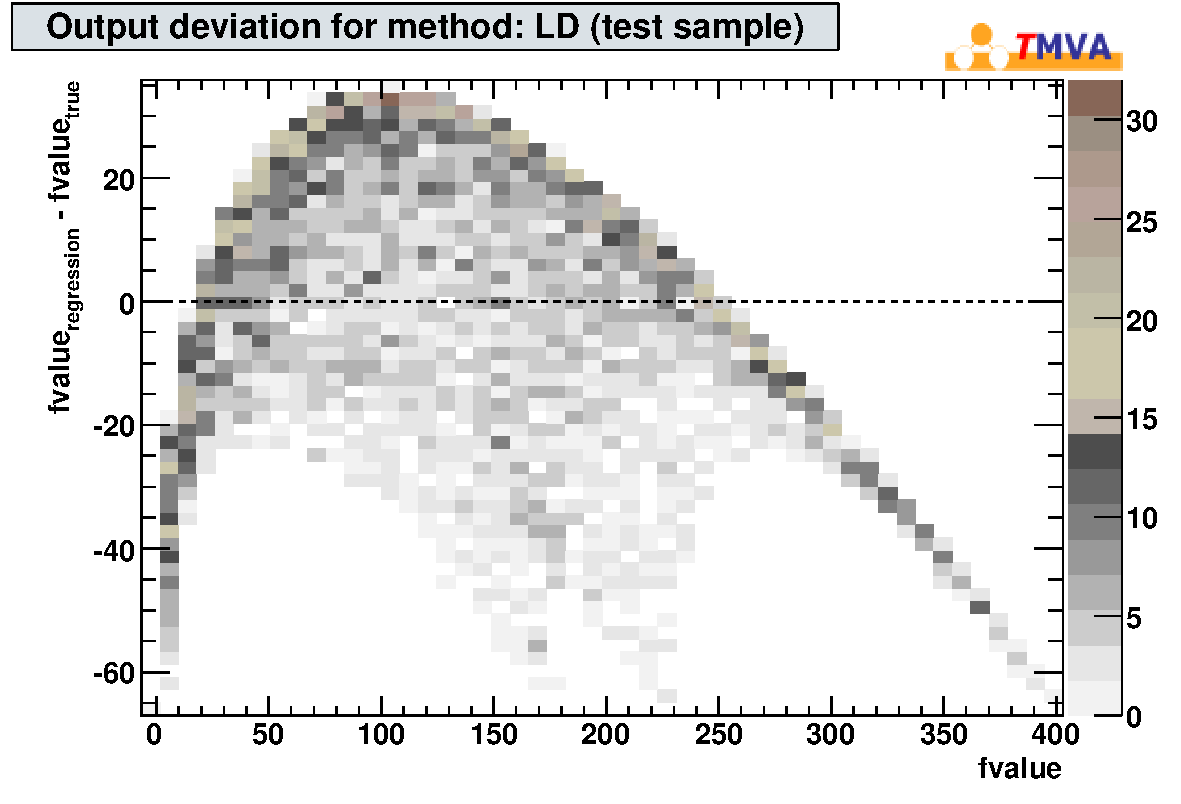
\includegraphics[width=0.50\textwidth]{plots/deviation_LD_target_test_c0}
  \hspace{-0.3cm}
  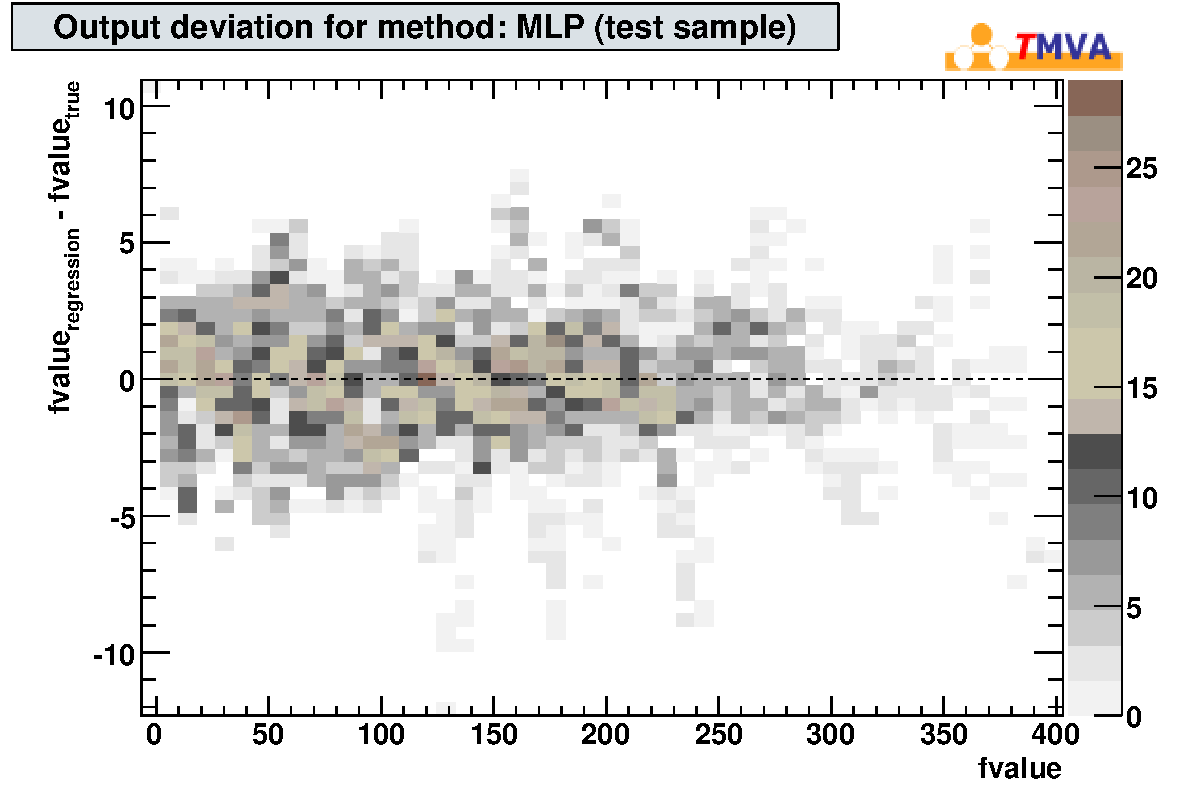
\includegraphics[width=0.50\textwidth]{plots/deviation_MLP_target_test_c0}
  \vspace{0.2cm}
\end{center}
\vspace{-1.2cm}
\caption[.]{Example plots for the deviation between regression output and target values
            for a Linear Discriminant (LD -- left) and MLP (right). The dependence of the 
            input variables on the target being strongly nonlinear, LD cannot appropriately 
            solve the regression problem. }
\label{fig:usingtmva:deviation}
\end{figure}



\subsection{Getting help}

Several help sources exist for TMVA (all web address given below are also linked from the 
TMVA home page \urlsm{http://tmva.sourceforge.net}).
\begin{itemize}

\item Information on how to download and install TMVA, and the TMVA {\em Quick-start} commands 
      are also available on the web at: \urlsm{http://tmva.sourceforge.net/howto.shtml}.

\item TMVA tutorial: \urlsm{https://twiki.cern.ch/twiki/bin/view/TMVA}.

\item An up-to-date reference of all configuration options for the TMVA Factory, the fitters,
      and all the MVA methods: \urlsm{http://tmva.sourceforge.net/optionRef.html}.

\item On request, the TMVA methods provide a help message with a brief description of the 
      method, and hints for improving the performance by tuning the available configuration 
      options. The message is printed when the option "\code{H}" is added to the configuration 
      string while booking the method (switch off by setting "\code{!H}"). The very same help
      messages are also obtained by clicking the ``info'' button on the top of the reference
      tables on the options reference web page: \urlsm{http://tmva.sourceforge.net/optionRef.html}.      

\item The web address of this Users Guide:
      \urlsm{http://tmva.sourceforge.net/docu/TMVAUsersGuide.pdf}.

\item The TMVA talk collection: \urlsm{http://tmva.sourceforge.net/talks.shtml}.

\item TMVA versions in ROOT releases: 
      \urlsm{http://tmva.sourceforge.net/versionRef.html}.

\item Direct code views via ViewVC: \urlsm{http://tmva.svn.sourceforge.net/viewvc/tmva/trunk/TMVA}.

\item Class index of TMVA in ROOT: \urlsm{http://root.cern.ch/root/htmldoc/TMVA_Index.html}.

\item Please send questions and/or report problems to the {\em tmva-users} mailing list: \\
      \urlsm{http://sourceforge.net/mailarchive/forum.php?forum_name=tmva-users} (posting 
      messages requires prior subscription: 
      \urlsm{https://lists.sourceforge.net/lists/listinfo/tmva-users}).

\end{itemize}

%%% Local Variables: 
%%% mode: latex
%%% TeX-master: "TMVAUsersGuide"
%%% End: 

